\documentclass[12pt]{article}
\usepackage[margin=2.5cm]{geometry}
\usepackage{enumerate}
\usepackage{amsfonts}
\usepackage{amsmath}
\usepackage{fancyhdr}
\usepackage{amsmath}
\usepackage{amssymb}
\usepackage{amsthm}
\usepackage{mdframed}
\usepackage{graphicx}
\usepackage{subcaption}
\usepackage{adjustbox}
\usepackage{listings}
\usepackage{xcolor}
\usepackage{booktabs}
\usepackage[utf]{kotex}
\usepackage{hyperref}

\definecolor{codegreen}{rgb}{0,0.6,0}
\definecolor{codegray}{rgb}{0.5,0.5,0.5}
\definecolor{codepurple}{rgb}{0.58,0,0.82}
\definecolor{backcolour}{rgb}{0.95,0.95,0.92}

\lstdefinestyle{mystyle}{
    backgroundcolor=\color{backcolour},
    commentstyle=\color{codegreen},
    keywordstyle=\color{magenta},
    numberstyle=\tiny\color{codegray},
    stringstyle=\color{codepurple},
    basicstyle=\ttfamily\footnotesize,
    breakatwhitespace=false,
    breaklines=true,
    captionpos=b,
    keepspaces=true,
    numbers=left,
    numbersep=5pt,
    showspaces=false,
    showstringspaces=false,
    showtabs=false,
    tabsize=1
}

\lstset{style=mystyle}

\pagestyle{fancy}
\renewcommand{\headrulewidth}{0.4pt}
\lhead{CSC 209}
\rhead{Review 7 Solution}

\begin{document}
\title{CSC 209 Review 7 Solution}
\maketitle

\bigskip

\section{Exercises}

\begin{enumerate}[1.]
    \item

    First, I need to justify if the folllowing declarations legal on an individual basis:

    \bigskip

    \texttt{struct \{int x, y;\} x;}

    \texttt{struct \{int x, y;\} y;}

    \bigskip

    The struct \texttt{struct \{int x, y;\} x;} is legal. \texttt{struct \{int x, y;\} x;}
    is equivalent to

\begin{lstlisting}[language=c]
    struct {
        int x;
        int y;
    } x;
\end{lstlisting}

    and `x' beside struct represents variable of that type. It is used to declare struct
    and access members of the struct (e.g. \texttt{x.x},, \texttt{x.y}).

    \bigskip

    The same is true for \texttt{struct \{int x, y;\} y;}.

    \bigskip

    Second, I need to answer if both declarations of struct can appear in a program.

    \bigskip

    The answer is yes. Each structure has a separate name space for it's members.

    \bigskip

    \underline{\textbf{Notes}}

    \begin{itemize}
        \item \textbf{Declaring Structure Variables}

        \begin{itemize}
            \item Struct can have many variables that represent the same struct

            \bigskip

            \begin{center}
            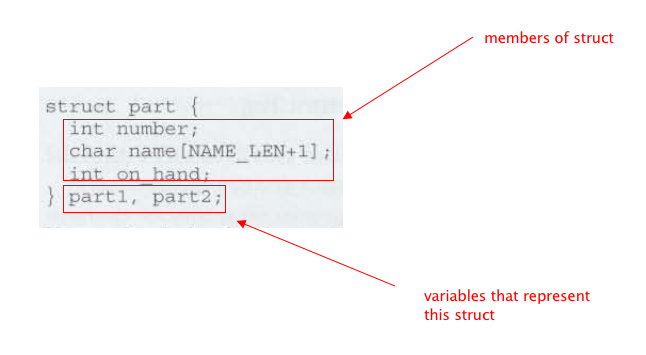
\includegraphics[width=0.8\linewidth]{images/review_7_solution_1.png}
            \end{center}
        \end{itemize}

        \bigskip

        \item \textbf{Initializing Structure Variables}

        \begin{itemize}
            \item Struct can be initialized with preset values (like python class under \_\_init\_\_)

            \bigskip

            \begin{center}
            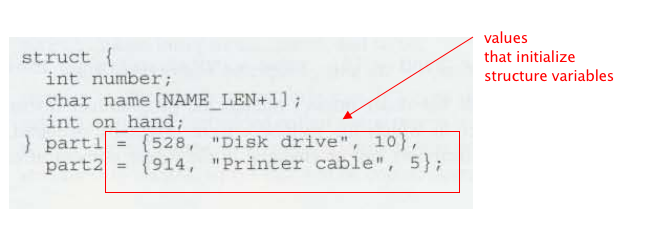
\includegraphics[width=0.8\linewidth]{images/review_7_solution_2.png}
            \end{center}

        \end{itemize}
    \end{itemize}

    \item

    \begin{enumerate}[a)]
        \item

        I need to declare structure variables named \texttt{c1}, \texttt{c2} and \texttt{c3},
        each having members \texttt{real} and \texttt{imaginary} of type \texttt{double}.

        \bigskip

        The solution to this problem is:

        \bigskip

\begin{lstlisting}[language=c]
    struct {
        double real, imaginary;
    } c1, c2, c3;
\end{lstlisting}

        \item

        I need to modify the declaration in part a) so that

        \begin{itemize}
            \item \texttt{c1}'s members initially have the values 0.0 and 1.0
            \item \texttt{c2}'s members initially have the values 1.0 and 0.0
            \item \texttt{c3} is not initialized
        \end{itemize}

        \bigskip

        The solution to this problem is:

        \bigskip

\begin{lstlisting}[language=c]
    struct {
        double real, imaginary;
    } c1 = {0.0, 1.0},
      c2 = {1.0, 0.0},
      c3;
\end{lstlisting}

        \bigskip

        \underline{\textbf{Notes}}

        \begin{itemize}
            \item \textbf{Designated Initializer}

            \begin{itemize}
                \item Allows specific member variable to be initialized
                \item Allows member variables to be initialized in any order
            \end{itemize}

            \bigskip

            \underline{\textbf{Example}}

            \bigskip

            \begin{center}
            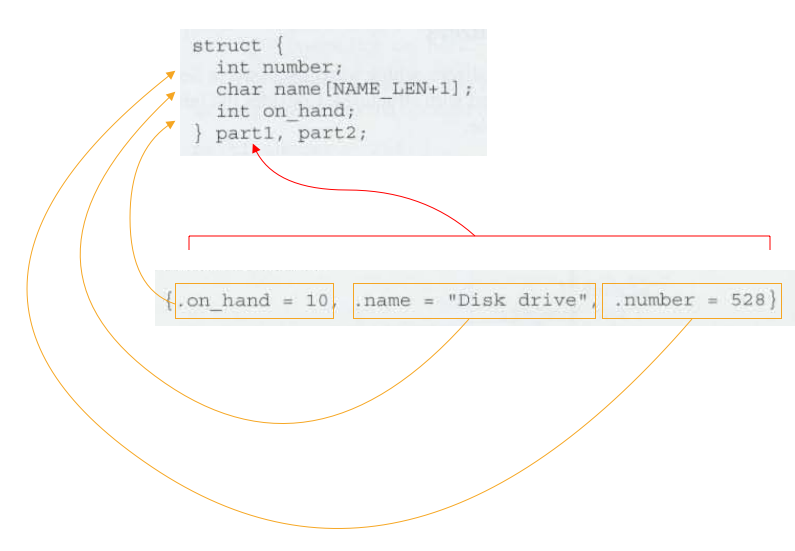
\includegraphics[width=0.8\linewidth]{images/review_7_solution_3.png}
            \end{center}
        \end{itemize}

        \item

        I need to write statements that copy the members of \texttt{c2} to \texttt{c1}.

        \bigskip

        Copying the members of \texttt{c2} and {c1} can be done in one statement.

        \bigskip

        Below is the solution to this problem:

        \bigskip

\begin{lstlisting}[language=c]
    c2 = c1
\end{lstlisting}

        \item

        I need to write statements that add the corresponding members of \texttt{c1}
        and \texttt{c2} and store the result in \texttt{c3}.

        \bigskip

        The solution to this problem is:


\begin{lstlisting}[language=c]
    struct {
        double real, imaginary;
    } c1 = {0.0, 1.0},
        c2 = {1.0, 0.0},
        c3;

    ...

    c3 = c1 + c2;
\end{lstlisting}

        \bigskip

        \underline{\textbf{Notes}}

        \begin{itemize}
            \item member variables of struct contains two operators \& and \texttt{.} (e.g \&\texttt{part1.number} and \texttt{part1.number})
            \item \& accesses memory address of the member variable, where as \texttt{.} accesses value
            \item \texttt{part1 = part2} \underline{copies} contents in \texttt{part2} to corresponding
            member variable in \texttt{part1}

            \bigskip

            \begin{center}
            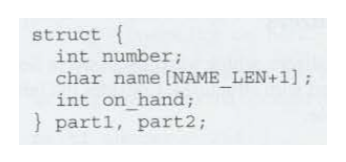
\includegraphics[width=0.5\linewidth]{images/review_7_solution_4.png}
            \end{center}
        \end{itemize}

    \end{enumerate}

    \item

    \begin{enumerate}[a)]
        \item

        I need to declare a tag named \texttt{complex} for a structure with two members
        \texttt{real} and \texttt{imaginary}, of type \texttt{double}

        \bigskip

        The solution to this problem is:

        \bigskip

\begin{lstlisting}[language=c]
    struct complex {
        double real, imaginary;
    };
\end{lstlisting}


        \underline{\textbf{Notes}}

        \begin{itemize}
            \item \textbf{Declaring a Structure Tag}

            \begin{itemize}
                \item allows to use struct in function calls
                \item allows to use the same struct in multiple files of a program
            \end{itemize}

            \bigskip

            \begin{center}
            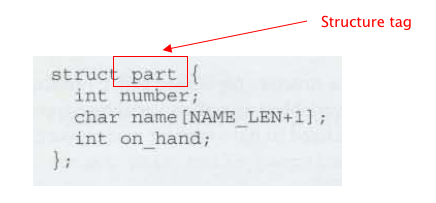
\includegraphics[width=0.6\linewidth]{images/review_7_solution_5.png}
            \end{center}
        \end{itemize}

        \item

        I need to use the \texttt{complex} tag to declare variables named \texttt{c1},
        \texttt{c2}, \texttt{c3}.

        \bigskip

        The solution to this problem is:

        \bigskip

\begin{lstlisting}[language=c]
    struct complex {
        double real, imaginary;
    } c1, c2, c3;
\end{lstlisting}

        \item

        I need to write a function named \texttt{make\_complex} that satisfies the following:

        \begin{itemize}
            \item The function \texttt{make\_complex} should have two parameters (\texttt{real}, \texttt{imaginary}) of type \texttt{double}
            \item The function \texttt{make\_complex} should store the two arguments in \texttt{complex} struct
            \item The function \texttt{make\_complex} should return the struct
        \end{itemize}

        \bigskip

        The solution to this problem is:

        \bigskip

\begin{lstlisting}[language=c]
    struct complex {
        double real, imaginary;
    };

    struct complex (double real, double imaginary) {
        struct complex c1;

        c1.real = real;
        c1.imaginary = imaginary;

        return c1;
    }
\end{lstlisting}

        \bigskip

        \underline{\textbf{Notes}}

        \begin{itemize}
            \item
        \end{itemize}
    \end{enumerate}
\end{enumerate}

\end{document}